\section{Task: Manage Sectors}
\label{sec:task_manage_sectors} 

This task allows management of sectors (as in 2.5D polygons) stored in the database. It can not be run, but is performed using the GUI elements. \\

It is recommended if the sectors are to be used for data processing and/or if the altitude information is of use. For 2D display-only polygons it is recommended to add such information to the used map files, as described in \nameref{sec:adding_maps}.

\begin{figure}[H]
  \hspace*{-2.5cm}
    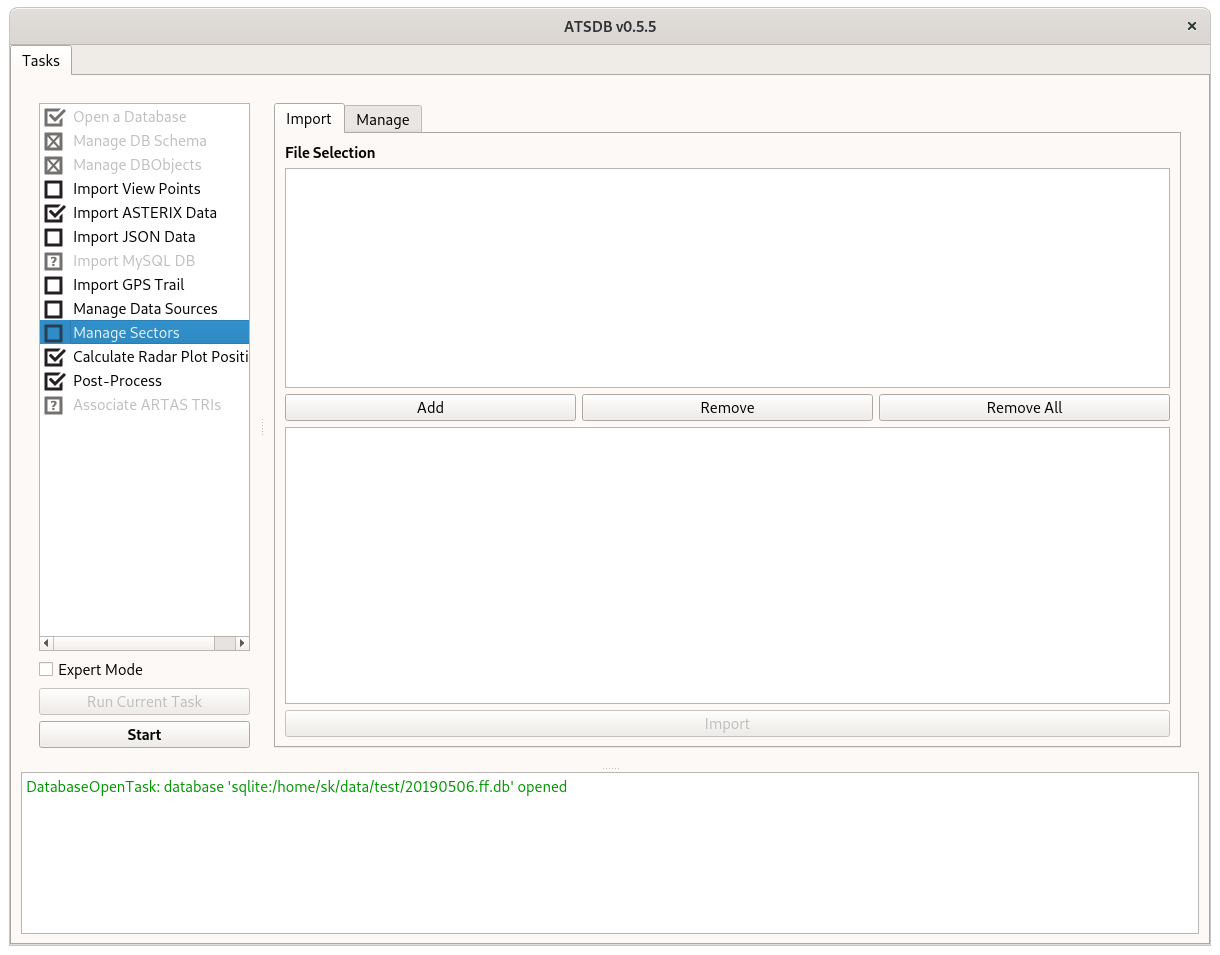
\includegraphics[width=19cm]{../screenshots/manage_sectors.png}
  \caption{Task: Manage Sectors}
\end{figure}

There exist 2 tabs:

\begin{itemize}  
\item Import: For importing sectors from files
\item Manage: Management of imported sectors stored in the database
\end{itemize}
\ \\

\paragraph {Import Tab}

In the 'File Selection' list, a list of available files is given. Entries can be added using the 'Add' button or removed using either the 'Remove' or 'Remove All' buttons. \\

Files are imported using the GDAL library, which can read a number of GIS files, and all encapsulated polygons or multi-polygons are written to the database with unique names. Supported common file-formats are e.g.:

\begin{itemize}  
\item ESRI Shapefile
\item GML
\item KML
\end{itemize}
\ \\

Note that only polygon information is added, and all information is assumed to be stored in the WGS84 coordinate system. \\

Below a text field is given which, after selection of a file, displays the content information and/or error messages. \\\

\paragraph {Manage Tab}

\begin{figure}[H]
    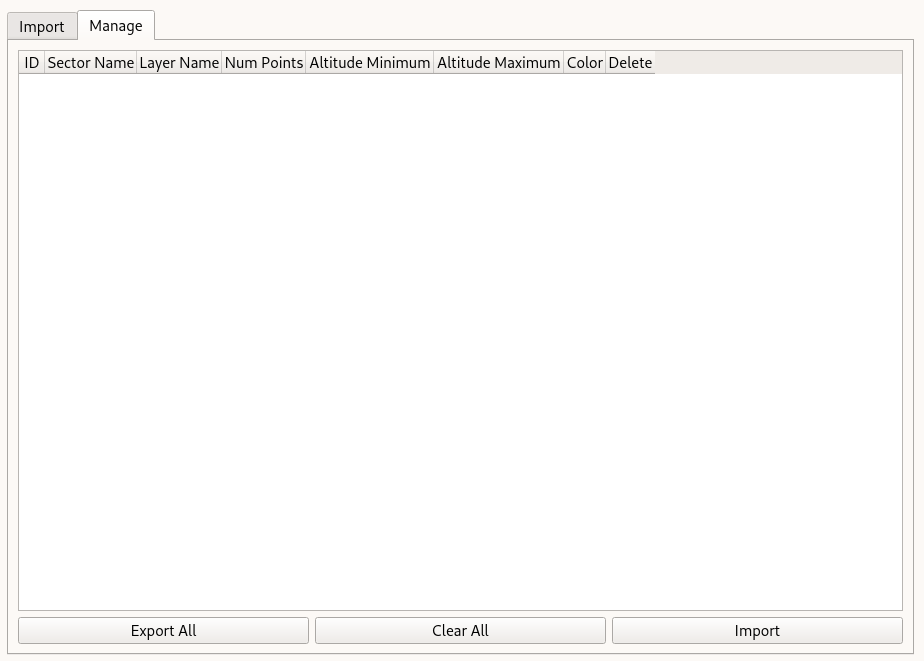
\includegraphics[width=16cm,frame]{../screenshots/manage_sectors_manage.png}
  \caption{Task: Manage Sectors Manage Tab}
\end{figure}

In the Manage tab, a table listing the existing sectors is given, which allows editing/deleting of the information stored in the database. \\

The following columns exist in the table:
\begin{itemize}  
\item ID: Unique identifier number, read-only
\item Sector Name: Name of the sector, editable
\item Layer Name: Name of the layer the sector will be grouped in, editable
\item Num Points: Number of points in polygon, read-only
\item Altitude Minimum: Minimum altitude in feet, editable, can be empty (gray)
\item Altitude Maximum: Maximum altitude in feet, editable, can be empty (gray)
\item Color: Color in display, editable
\item Delete: Delete button
\end{itemize}
\ \\

At the botton, 3 buttons exist:

\begin{itemize}  
\item Export All: Saves all stored sectors as JSON file
\item Clear All: Deletes all stored sectors
\item Import: Imports a previously exported sector JSON file
\end{itemize}
\ \\

\paragraph {Running}

After adding two example files, the 'Import' tab looks as follows:

\begin{figure}[H]
    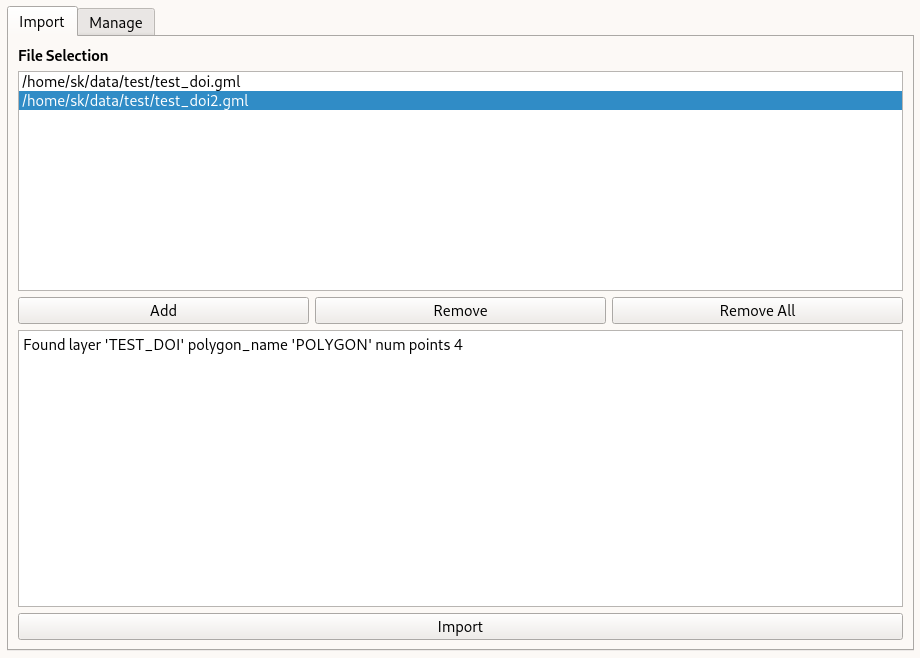
\includegraphics[width=16cm,frame]{../screenshots/manage_sectors_ready.png}
  \caption{Task: Manage Sectors with Example Files}
\end{figure}

To import a sector, select the wanted file in the file list and press the 'Import' button. After successful import, a confirmation message is shown. \\

After importing both sectors, the 'Manage' tab looks as follows:

\begin{figure}[H]
    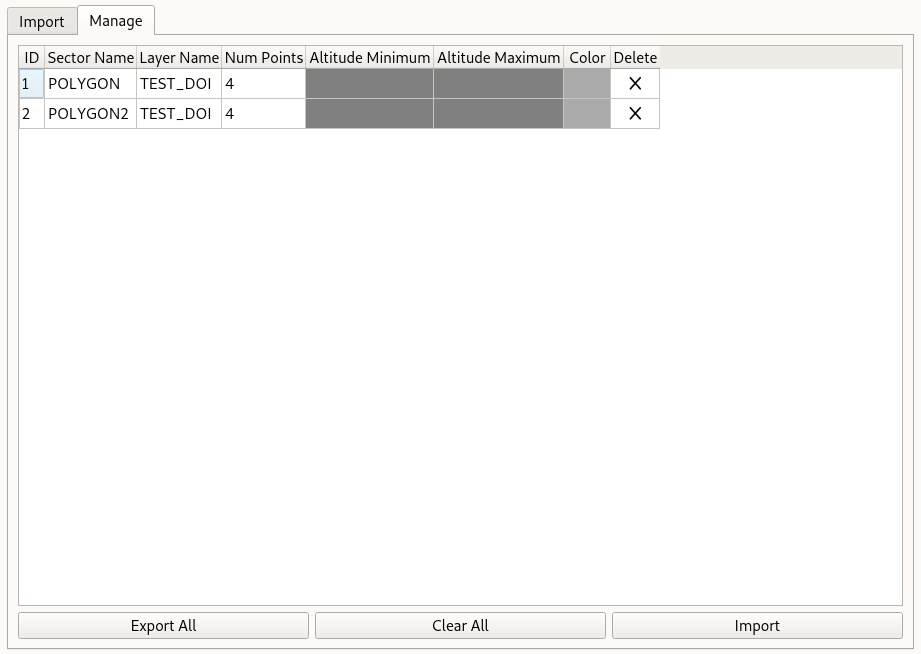
\includegraphics[width=16cm,frame]{../screenshots/manage_sectors_manage2.png}
  \caption{Task: Manage Sectors with Example Sectors}
\end{figure}

The attributes of the respective sector can be changed as wanted, by double-clicking on the text value or clicking on the color. Each change is stored immideately in the database. \\

It is recommended to export all sectors after creation, for later usage (e.g. in another database).

